\documentclass{article}

% if you need to pass options to natbib, use, e.g.:
%     \PassOptionsToPackage{numbers, compress}{natbib}
% before loading neurips_2020

% ready for submission
% \usepackage{neurips_2020}

% to compile a preprint version, e.g., for submission to arXiv, add add the
% [preprint] option:
%     \usepackage[preprint]{neurips_2020}

% to compile a camera-ready version, add the [final] option, e.g.:
%     \usepackage[final]{neurips_2020}

% to avoid loading the natbib package, add option nonatbib:
     \usepackage[nonatbib]{neurips_2020}

\usepackage[utf8]{inputenc} % allow utf-8 input
\usepackage[T1]{fontenc}    % use 8-bit T1 fonts
\usepackage{hyperref}       % hyperlinks
\usepackage{url}            % simple URL typesetting
\usepackage{booktabs}       % professional-quality tables
\usepackage{amsfonts}       % blackboard math symbols
\usepackage{nicefrac}       % compact symbols for 1/2, etc.
\usepackage{microtype}      % microtypography
\usepackage{graphicx}
\usepackage{multicol}
\usepackage{subfig}
\graphicspath{ {./} }
\usepackage{float}
\usepackage{biblatex}
\usepackage{subcaption}
\usepackage[]{graphicx}


\addbibresource{citations.bib}

\usepackage{booktabs}
\usepackage{multirow}
\usepackage{siunitx}



\title{STA 640: Bayesian Non-Parametric Analysis of Heterogenous Treatment Effects.}

% The \author macro works with any number of authors. There are two commands
% used to separate the names and addresses of multiple authors: \And and \AND.
%
% Using \And between authors leaves it to LaTeX to determine where to break the
% lines. Using \AND forces a line break at that point. So, if LaTeX puts 3 of 4
% authors names on the first line, and the last on the second line, try using
% \AND instead of \And before the third author name.

\author{%
  David S.~Hippocampus\thanks{Use footnote for providing further information
    about author (webpage, alternative address)---\emph{not} for acknowledging
    funding agencies.} \\
  Department of Computer Science\\
  Cranberry-Lemon University\\
  Pittsburgh, PA 15213 \\
  \texttt{hippo@cs.cranberry-lemon.edu} \\
  % examples of more authors
  % \And
  % Coauthor \\
  % Affiliation \\
  % Address \\
  % \texttt{email} \\
  % \AND
  % Coauthor \\
  % Affiliation \\
  % Address \\
  % \texttt{email} \\
  % \And
  % Coauthor \\
  % Affiliation \\
  % Address \\
  % \texttt{email} \\
  % \And
  % Coauthor \\
  % Affiliation \\
  % Address \\
  % \texttt{email} \\
}

\begin{document}

\maketitle

\begin{abstract}
  In this paper I propose the use of Ewens-Pitman Attraction (EPA) regression, to perform Bayesian non-parametric regression and clustering for the purpose of identifying treatment effect heterogeneity in randomized experiments. EPA regression is able to simultaneously fit a flexible regression model as well as discover partitions in the sample, the latter of which this work seeks to exploit in finding treatment effect heterogeneity.  
\end{abstract}

\section{Introduction}

One goal of heterogeneous treatment effect (HTE) analysis is to examine if a treatment affects an individual or population subgroup more then others. Identifying such treatment effect heterogeneity is crucial since average or marginal treatment effects may mask the effect of a policy. For example, a subgroup may have a negative treat effect to a medicine whereas the ATE might be positive, it is thus crucial that methods be available to identify such groups. 
\\ \\
The typical approach to HTE analysis is through the use of subgroup analysis. Subgroups are partitions of the covariate space, and are typically pre-specified based on domain knowledge. For example we might specify a males vs females subgroup, and compare difference in treatment effect between the groups. This provides the first motivation for the application of bayesian non-parametric modelling, that such subgroups can be inferred from the data instead of being pre-specified. This is important for several reasons, firstly domain expertise might not be available to specify the subgroups, secondly even with domain expertise a cluster analysis can often times still provide valuable insights into the data, lastly cluster analysis can be useful in finding subgroups in higher dimensions.
\\ \\ 
Besides identifying subgroups, another key part of HTE is that of modelling the Conditional Average Treatment Effect (CATE). In general this can be done several ways, such as with weighting with an IPW estimator. For this work we focus on the outcome modelling approach, where a model is fit to estimate outcomes under all treatment arms. This approach then provides the second motivation for using a bayesian non-parametric approach. Bayesian non-parametrics provides one avenue to specify flexible regression models. In this case, the regression model used is a mixture of linear regression models, where the number of mixture components is dynamic. 
\\ \\
To achieve both aims, a bayesian non-parametric regression model built on the Ewens-Pitman Attraction (EPA) distribution is used (cite chris glynn and dalh). The EPA distribution is a distribution on partitions indexed by a pairwise similarity function (make it nicer). For our application, such similarity is based on the distances between covariates in which we are interested in analysing HTE over. Intuitively, data points with higher similarity in covariates are apriori more likely to be clustered together. EPA regression combines the EPA distribution with a regression sampling model, allowing one to fit a mixture of regressions where data points are allocated to different clusters based on how well a clusters associated parameters can explain a data points outcome - covariate relationship, and its covariate - covariate relationship vis-a-via other points in the cluster. Being a non-parametric clustering model, it also shares the same property as models like the Dirichlet Process mixture model and Pitman Yor mixure model, in that points that are not well explained by existing clusters can start new clusters. In theory, this implies that the model also helps select for the number of clusters, an aspect that is often left as a hyperparameter in most clustering algorithms.
\\ \\ 
\section{Related Work}

The EPA regression model is based off (Dahl), and we apply it to the problem of heterogenous treatment effect. In their work, they showed that the model is able to do latent subgroup regression... and is able to outperform ... . This motivates the use of EPA regression over similar partition distributions. 

Another similar application of EPA regression is in glynn, which applies the EPA regression model to modelling homeless rates across various continum of care. Here the authors posit that CoCs are likely to be similar to each other.., motivating the use of EPA regression. A key difference however is that the work does not aim to find a causal effect, likely due to the fact that their data is largely observational. 

Lastly, the work of causal clustering in [], also seeks to discover latent subgroups in the data. The approach however is different. With causal clustering the author first uses an outocme model to estimate the vector of potential outcomes. These estimated potential outcomes are passed into a clustering algorithm like K-means or hierarchical clustering in order to find clusters of data points in the potential outcome space. These clusters, if they exist are likely to have differing levels treatment effect. Our work is different in that we exploit the EPA regression model's ability to model and cluster jointly, bypassing the need to fit outcome and clustering model separately. 

\section{Model}
\label{sec:Model}
\paragraph{Causal Estimand and Setup} We consider either an observational or randomized control trial consisting of $n$ iid samples. Each sample $i$ is an tuple $(Y_i, D_i, X_i, Z_i)$. Where $Y_i$ is the treatment outcome, $D_i$ is the assigned treatment, $X_i$ are covariates and $Z_i$ are variables we seek to perform HTE analysis over. Note that it is generally the case that $Z_i = X_i$ or $Z_i$ is a subset of the variables in $X_i$. We further consider the case of a continuous outcome, that is $Y_i$ is continuous and a binary treatment, that is $D_i \in {0,1}$. $X_i$ and $Z_i$ are vectors $d$ and $p$ dimenionsal vectors and can be of mixed continuous and categoricals elements. For treatment effect identification with have the following assumptions.
\begin{itemize}
    \item SUTVA: ...
    \item Positivity ... 
    \item No unmeasured confounding ...
\end{itemize}
For randomized control trials, assumption A3 is automatically fulfilled due to the randomized nature of treatment assignment $D_i$. For observational studies, A3 implies that any confounders of $D_i$ and $Y_i$ are observed in the set $X_i$. 
\\ \\
The causal quantity of interest is the conditional average treatment effect (CATE) given by:
$$CATE(X) = E[Y(1)-Y(0)|X]$$ 
\\ 
Under the assumptions, CATE can be identified as:
$$E[Y(1)-Y(0)|X] = E[Y|D=1] - E[Y|D=0]$$ 
\\ 
Thus the modelling approach is to specify models for $E[Y|D=1]$ and $E[Y|D=0]$. For this work, we take the S-learner approach, where a single model $Y=f(D,X)$ is specified and we take $f(1,X) = E[Y|D=1]$ and $f(0,X) = E[Y|D=0]$. The estimator for CATE is then:
$$\hat{CATE(X)} = f(1,X) - f(0,X)$$ 
where $f$ is the EPA regression model.

\paragraph{EPA Distribution}
The EPA distribution is a distribution over partitions indexed by a pairwise similarity function. That is, suppose we have points $X_1,...,X_n$ and a similarity function $\lambda(X_i,X_j)$. Denote $s={s_1,...,s_n}$ a partition of the dataset. The EPA distribution can be written as a product of pairwise probabilities. 

\begin{equation}
\label{eqn:EPA Distribution}
P(\pi_1) = ..
\end{equation}
\\ Where each $P_i(t) is given by.$
\begin{equation}
\label{eqn:EPA Distribution}
P(\pi_1) = ..
\end{equation}

\paragraph{Outcome Model}

\paragraph{Model Inference} 
Inference proceeds by way of a Gibbs - Sampler over the parameters $\pi$, $\phi$, $\alpha$, $order$ and $\beta$. For $\pi$ the gibbs sample iterates over each data point. Proposing for each data point a possible move to other existing clusters, or starting a new cluster. This is given by :
#insert equation


\section{Data}

We experiment with two datasets. A simulated dataset as well as the National Supported Work Demonstration (NSW) dataset.

\paragraph{Simulated Dataset} This dataset consists of xx simulated data points from 3 latent regression functions. Index these latent regression functions by 1,2,3 respectively. We firstly generate 1D covariates $X_k$ from Gaussian distributions centered at x x and x with standard deviations x x and x. For each cluster $k$ x points are generated. Then we specify 3 regression functions.

\begin{equation}
\label{eqn:latent_reg1}
Y_{i1} = 0.3 * D_{i1} + 0.5*X_{i1} + 0.6*X_{i1}*D_{i1} + \sigma_1
\end{equation}
\begin{equation}
\label{eqn:latent_reg1}
Y_{i2} = 0.3 * D_{i2} + 0.5*X_{i2} + 0.6*X_{i2}*D_{i2} + \sigma_2
\end{equation}
\begin{equation}
\label{eqn:latent_reg1}
Y_{i3} = 0.3 * D_{i3} + 0.5*X_{i3} + 0.6*X_{i3}*D_{i3} + \sigma_3
\end{equation}

Each treated $D_ik$ is generated at random with $P(D_ik) = 0.5$, meaning that treatment in this simulated dataset is randomly assigned. Lastly the values of $Y_{ik}$ are generated based one generated $X_{ik}$ and the randomly assigned $D_{ik}$. A plot of the dataset can be seen in figure xx. 

\paragraph{National Supported Work Demonstration (NSW) Data} The National Supported Work Demonstration job training was a experimental program ran in the 1970s by Manpower Demonstration Research Corp (MRDC). The program involved giving participants temporary employment which was designed to help those lacking basic job skills move into the labor market by giving them work experience. The dataset consists of 405 individuals along with x covariates consisting of demographic information, educational background as well as income levels prior to the program. The outcome we measure is the income level post the program. 
\\ \\ 
For the NSW data, we take a further subset of xx individuals who are employed at the end of the program period (whether they were treated or not), this is for computational reasons, with the 0 data points affecting the gaussian likelihood. It is important to note however that effects estimated here are thus not representative of the population that the NSW data sets out to measure the policies effectiveness over.


\section{Modelling and Results}
In this section we discuss the modelling details for each dataset as well as the results. 
\\ \\
\subsection{Modelling Parameters}
\paragraph{Simulated Data}
For the simulated dataset, we fit the EPA regression model with a Gaussian likelihood and interaction effects. That is:
$$Y_i = \beta_{0k} + \beta_{1k}D_i + \beta_{2k}X_i + \beta_{3k}X_iD_i$$
\\ \\
We fixed the regression error $\sigma$ as 1. The prior on $\alpha$ is a $Ga(1,10)$ distribution, and the prior on $\beta$ is a mixture of a point mass at 0 and a $\beta(1,1)$ distribution, with each mixture component having an identical weight of 0.5. The prior on $\phi$ is a multivariate normal with 0 mean and an identity matrix as the covariance.  For this model we generated a total of 10000 gibbs sample, with 5000 being discarded as burn-in. 

\paragraph{NSW Data} For the NSW data, we fit EPA regression model with a Gaussian likelihood but without interaction effects. That is:
$$Y_i = \beta_{0k} + \beta_{1k}D_i + \beta_{2k}X_i$$, where $X_i$ is a vector of covariates. We remove interaction effects as we find it results in too many parameters, leading to poor fit of the model. Further we transform the outcome $Y$ by analysing in 1000s that is dividing $Y$ by 1000. This is to avoid having to set large prior values for $\phi$ parameters.
\\ \\
Prior distributions on $\alpha$ and $\beta$ is identical to that used for the model on the simulated data. For $\phi$ we use a zero-mean Gaussian distribution, with a diagonal covariance matrix. This covariance has 1s in all diagonal elements except for the intercept term and the treatment treat, for which the prior variance are 3 and 2 respectively. For this model we generated a total of 15000 gibbs sample, with 5000 being discarded as burn-in. 

\subsection{Simulated Dataset Results} 
For the simulated data, we know the underlying latent clusters and associated regression function for each data point. We thus benchmark the model based how close the model estimated clustering is to the ground truth clusters. 

\paragraph{Obtaining Clusters} One issue to note is that our model outputs Monte Carlo samples of possible partitions. There is thus a need to post-process the set of samples to one coherent cluster assignment. For this we take the approach of cite which applies hierarchical clustering to the posterior similarity matrix. 
\\ \\
Using this approach, we find that (unsurprisingly) a 3 cluster solution is the most reasonable, that is 4,5 and 6 cluster solutions produced singleton clusters. Further looking at the posterior partition samples, we found that the average number of unique partitions is also 3. 
\\ \\
Fig X plots the obtained cluster solutions over the $Y^{obs}$ vs $X$ scatter plot. We see that the results almost perfectly match the true latent clustering, indicating the model is able to detect the latent clusters corresponding to the heterogeneous treatment effects. 
\\ \\
\paragraph{Predicting Potential Outcomes} We choose not to analyse parameters associated to each cluster due to label switching. Instead we analyse each cluster by looking at the mean predicted treatment effect for that cluster. For this we use the monte carlo samples to estimate for each individual $i$ the potential outcomes $Y_i(1)$ and $Y_i(0)$ as $\hat{f}(1,X)$ and $\hat{f}(0,X)$ respectively. Fig X plots the distribution of the ITEs separated by clusters. ... Analysis.

\subsection{NSW Dataset Results} 




\section{Conclusion}
In this work, we have explored the use of the Log Gaussian Cox Process to build a spatio-temporal Model of crime rates in Chicago. Two extensions, an Intrinsic Coregionalization Model for modelling multi-outputs and Kronecker Covariance, for scaling the model to larger datasets, were explored. The latter enabled us to fit the model various models within a reasonable amount of time, and with a reasonable amount of compute, whereas the former out-performed models where each crime type were fitted independently. Further, based on our benchmarking, we saw that the ICM extension was essential in building a predictive model which outperformed baseline's consistently. Overall, we have demonstrated that these Gaussian process models are both accurate, and also have the potential to scale, thus demonstrating the potential of their use in modelling the complex crime occurrence data. 




\appendix

\section{Simulated Data Plots}

\begin{figure}[h]
  \centering
  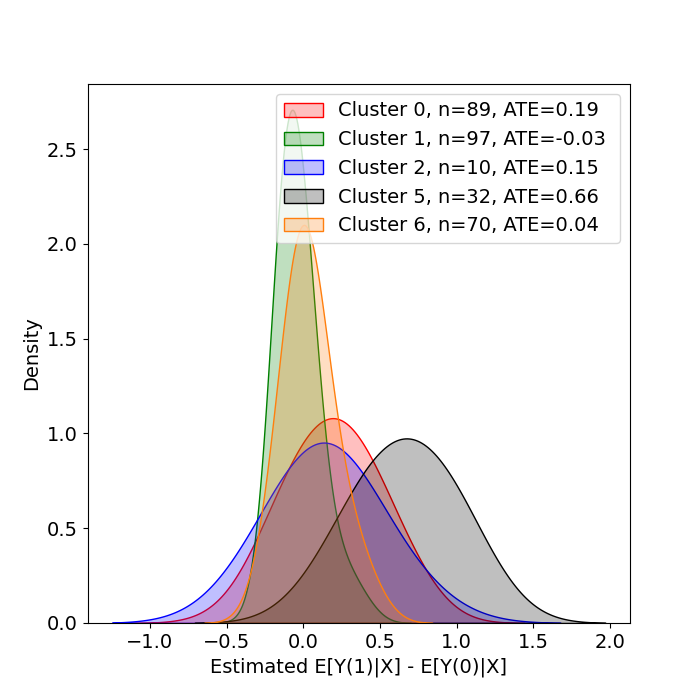
\includegraphics[width=0.8\textwidth]{Plots/NSW_output_histogram.png}
  \caption{This is a caption for the image.}
  \label{fig:sim_data_info}
\end{figure}

\section{Simulated Data Results}

\begin{figure}[H]
  \centering
  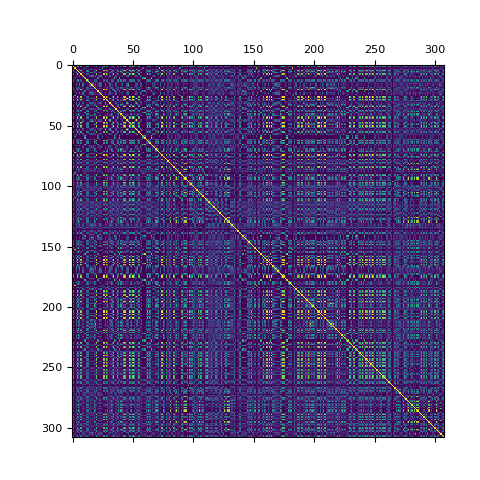
\includegraphics[width=0.8\textwidth]{Plots/NSW Posterior Similarity Matrix.png}
  \caption{Posterior similarity matrix inferred from simulated data}
  \label{fig:sim_post_mat}
\end{figure}

\begin{figure}[H]
  \centering
  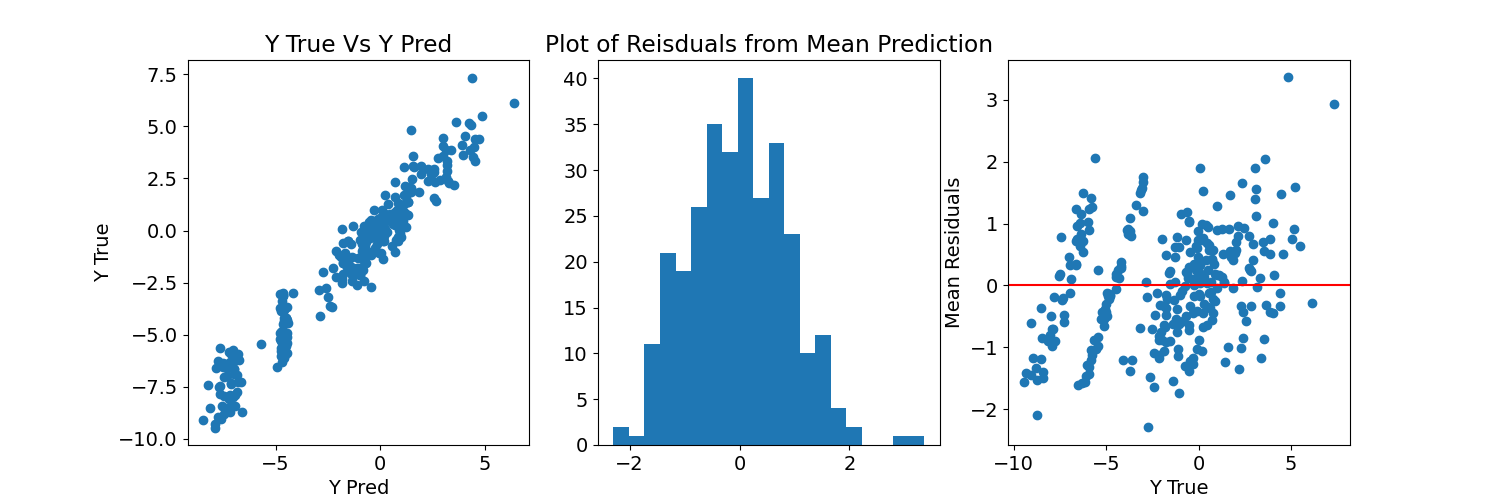
\includegraphics[width=1\textwidth]{Plots/simuated_diagnostics.png}
  \caption{Diagnostic Plots}
  \label{fig:sim_diag_plots}
\end{figure}

\begin{figure}[H]
  \centering
  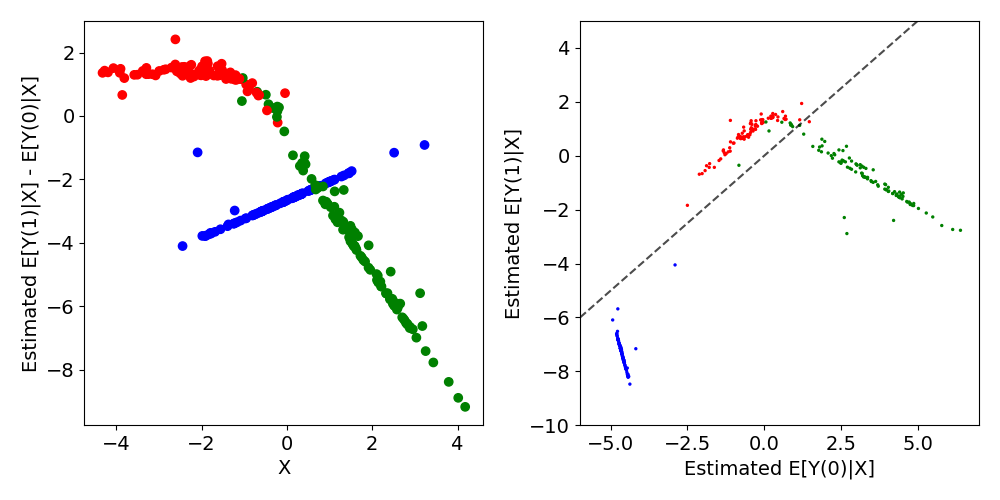
\includegraphics[width=1\textwidth]{Plots/Simulated_output_scatted.png}
  \caption{Scater plots}
  \label{fig:sim_scatter_plots}
\end{figure}

\begin{figure}[H]
  \centering
  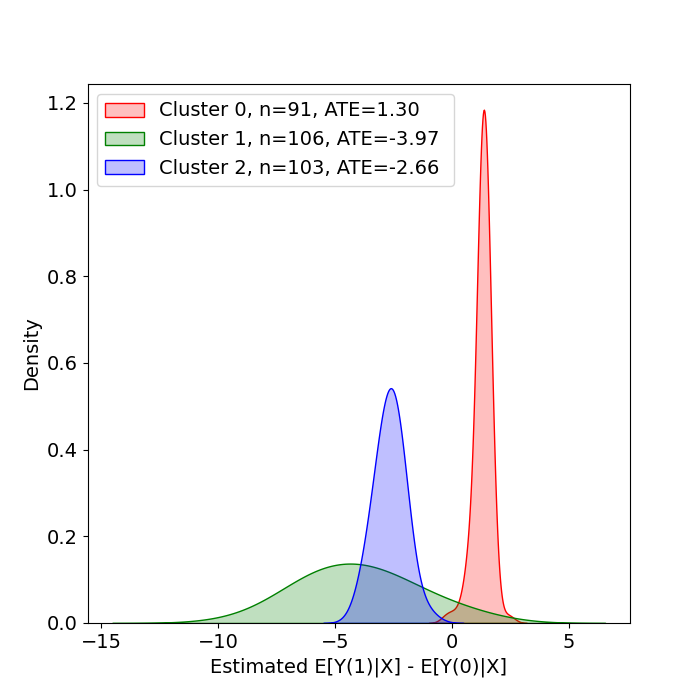
\includegraphics[width=0.8\textwidth]{Plots/Simulated_output_histogram.png}
  \caption{Simulated Data Histo}
  \label{fig:sim_histo}
\end{figure}



\section{NSW Data Results}

\printbibliography

\end{document}
